\subsection{Splitting axiom} \label{Subsection splitting}

In this section we consider certain boundary strata of the moduli space of quasimaps, called \ilemph{centipede loci}. These are the analogues in the absolute setting of the comb loci which appear in the relative setting (\S \ref{Subsection recursion formula for PN}). The general element of such a locus has a source curve with $r+1$ irreducible components, one ``trunk'' of the centipede and $r$ ``legs.'' Each of these components has a prescribed genus, curve class and set of marked points.

Given such a locus, there are two natural virtual classes with which it can be equipped. One is the product virtual class induced by the absolute product of the $r+1$ quasimap spaces, and the other is the class pulled back from the ambient moduli space. In this section we show that these classes coincide. This is the quasimap version of the \emph{splitting axiom} from Gromov--Witten theory, called the \emph{cutting edges axiom} in \cite{Behrend}.

We first establish notation. Fix a smooth projective toric variety $X$ and numerical invariants $g,n,\beta$ such that the corresponding quasimap space is defined. Now fix partitions $G=(g_0,\ldots,g_r)$ of the genus, $A=(A_0,\ldots,A_r)$ of the marked points and $B=(\beta_0, \ldots, \beta_r)$ of the curve class and consider the following space (which we call the \ildef{centipede locus}):
\begin{equation*} \D{X}{G,A}{B} := \Q{g_0}{A_0 \cup \{ q_1^0, \ldots, q_r^0 \}}{X}{\beta_0} \times_{X^r} \prod_{i=1}^r \Q{g_i}{A_i\cup\{q_i^1 \}}{X}{\beta_i} \end{equation*}
Of course we assume that every element of the partition is in the stable range, so that every factor in the above product makes sense. See Remark \ref{Remark on definition of comb locus} for a justification of why these are the correct boundary strata to consider. We can equip the centipede locus with the product virtual class in the following way. Set
\begin{equation*} \E{X}{G,A}{B} :=  \Q{g_0}{A_0 \cup \{ q_1^0, \ldots, q_r^0 \}}{X}{\beta_0} \times \prod_{i=1}^r \Q{g_i}{A_i\cup\{q_i^1\}}{X}{\beta_i} \end{equation*}
which we endow with the product class:
\begin{equation*} \virt{\E{X}{G,A}{B}} := \virt{\Q{g_0}{A_0 \cup \{ q_1^0, \ldots, q_r^0 \}}{X}{\beta_0}} \times \prod_{i=1}^r \virt{\Q{g_i}{A_i\cup\{q_i^1\}}{X}{\beta_i}} \end{equation*}
We then consider the cartesian diagram:
\begin{equation} \label{Product diagram}
\begin{tikzcd}
\D{X}{G,A}{B} \ar[r,"h"] \ar[d,"\ev_q"] \ar[rd,phantom,"\square"] & \E{X}{G,A}{B} \ar[d,"\ev_q"] \\
X^r \ar[r,"\Delta_{X^r}"] & X^r \times X^r
\end{tikzcd}
\end{equation}
Since $X$ is smooth $\Delta_{X^r}$ is a regular embedding, so we have a Gysin map which we use to define:
\begin{equation*} \virt{\D{X}{G,A}{B}} := \Delta_{X^r}^! \virt{\E{X}{G,A}{B}} \end{equation*}
Notice that if we set
\begin{equation*} \MM_{G,A,B}^{\operatorname{wt}} := \MM_{g_0,A_0\cup\{q_1^0,\ldots,q_r^0\},\beta_0}^{\operatorname{wt}} \times \prod_{i=1}^r \MM_{g_i,A_i\cup\{q_i^1\},\beta_i}^{\operatorname{wt}} \end{equation*}
then there is a morphism given by forgetting everything except the source curves and their classes
\begin{equation*} \rho_E : \E{X}{G,A}{B} \to \MM_{G,A,B}^{\operatorname{wt}} \end{equation*}
and the virtual class on $\E{X}{G,A}{B}$ is induced by a perfect obstruction theory $\EE_{\rho_E} \to \LL_{\rho_E}$ given by the product of the standard obstruction theories for each factor:
\begin{equation*} \Q{g_i}{A_i\cup\{q_i\}}{X}{\beta_i}\to \MM_{g_i,A_i,\beta_i}^{\operatorname{wt}} \end{equation*}
On the other hand, we have the following cartesian diagram
\begin{equation} \label{Full quasimap diagram}
\begin{tikzcd}
\D{X}{G,A}{B} \ar[r,"\varphi"] \ar[d,"\rho_D"] \ar[rd,phantom,"\square"] & \Q{g}{n}{X}{\beta} \ar[d,"\rho_Q"] \\
\MM_{G,A,B}^{\operatorname{wt}} \ar[r,"\psi"] & \MM_{g,n,\beta}^{\operatorname{wt}}
\end{tikzcd}
\end{equation}

The bottom horizontal map is not a closed immersion: due to the existence of degree--$0$ rational components, there may be many possible equally valid ways of breaking up a nodal curve. For instance, consider the following example of two elements which map to the same curve under $\psi$.

\begin{center}
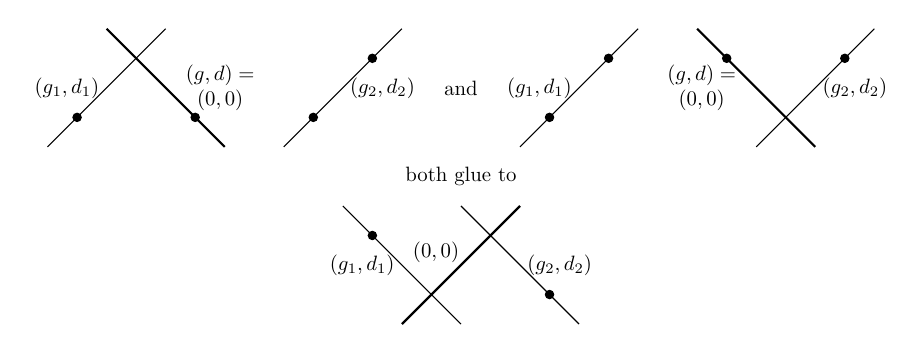
\begin{tikzpicture}[scale=.75,every node/.style={transform shape}]
  \draw (0,0) -- node[left]{$(g_1,d_1)$} (2,2);
  \draw[thick] (1,2) -- node[right]{\begin{tabular}{c} $(g,d)=$ \\ $(0,0)$ \end{tabular}} (3,0);
  \draw[fill=black] (.5,.5) circle[radius=2pt] (2.5,.5) circle[radius=2pt];
  \draw (4,0) -- node[right]{$(g_2,d_2)$}(6,2);
  \draw[fill=black] (4.5,.5) circle[radius=2pt] (5.5,1.5) circle[radius=2pt];
  
  \draw (7,1) node{and};
  
  \draw (8,0) -- node[left]{$(g_1,d_1)$} (10,2);
  \draw[fill=black] (8.5,.5) circle[radius=2pt] (9.5,1.5) circle[radius=2pt];
  \draw[thick] (11,2) -- node[left]{\begin{tabular}{c} $(g,d)=$ \\ $(0,0)$ \end{tabular}} (13,0);
  \draw (12,0) -- node[right]{$(g_2,d_2)$} (14,2);
  \draw[fill=black] (11.5,1.5) circle[radius=2pt] (13.5,1.5) circle[radius=2pt];

  \draw (7,-.5) node{both glue to};
  
  \draw (5,-1) -- node[left]{$(g_1,d_1)$}(7,-3) (7,-1) -- node[right]{$(g_2,d_2)$} (9,-3);
  \draw[thick] (6,-3) -- node[above left=-.1cm]{$(0,0)$} (8,-1);
  \draw[fill=black] (5.5,-1.5) circle[radius=2pt] (8.5,-2.5) circle[radius=2pt];
\end{tikzpicture}
\end{center}
Nevertheless $\psi$ has a natural perfect obstruction theory, given by $\LL_{\psi}$: we only need to show that it is supported in $[-1,0]$. Consider the exact triangle:
\begin{equation*} \psi^* \LL_{\MM_{g,n,\beta}^{\operatorname{wt}}} \to \LL_{\MM_{G,A,B}^{\operatorname{wt}}} \to \LL_\psi \xrightarrow{[1]} \end{equation*}
The first two terms are concentrated in degrees $[0,1]$, because they are the cotangent complexes of smooth Artin stacks. Therefore $\LL_\psi$ is concentrated in degrees $[-1,1]$. Furthermore, if we examine the long exact cohomology sequence near $\h^1(\LL_\psi)$ we find
\begin{equation*} \h^1(\psi^* \LL_{\MM_{g,n,\beta}^{\operatorname{wt}}}) \to \h^1(\LL_{\MM_{G,A,B}^{\operatorname{wt}}}) \to \h^1(\LL_\psi) \to 0 \end{equation*}
and hence we must show that the first map is surjective. But this is dual to the map which takes an infinitesimal automorphism of the disconnected curve to an infinitesimal automorphism of the corresponding connected curve (obtained by glueing together the ``nodal'' marked points). The space of infinitesimal automorphisms of a nodal curve splits into a direct sum of infinitesimal automorphisms of each component; since the glueing does not affect the components, we see that this map is an isomorphism. Hence $\h^1(\LL_\psi) = 0$ as claimed; morally this follows from the fact that the fibres of $\psi$ are Deligne--Mumford.

Hence there is a virtual pull-back map $\psi^!$ which defines a class
\begin{equation*}\psi^! \virt{\Q{g}{n}{X}{\beta}} \end{equation*}
on $\mathcal{D}^{\mathcal{Q}}(X,G,A,B)$. This is the same class as the one induced by the following perfect obstruction theory
\begin{equation*} \varphi^* \EE_{\rho_Q} \to \LL_{\rho_D} \end{equation*}
by functoriality of virtual pull-backs.

Finally if we look at \eqref{Product diagram} we see that $\ev_q^* \LL_{\Delta_{X^r}} \to \LL_h$ is a perfect obstruction theory for the map $h$. To summarise, we have a triangle
\begin{equation}\label{D-E-triangle}
 \begin{tikzcd}
  \D{X}{G,A}{B} \ar[dr,"\rho_D" below=0.1cm] \ar[rr,"h"] & & \E{X}{G,A}{B}\ar[dl,"\rho_E"] \\
& \MM_{G,A,B}^{\operatorname{wt}} &
 \end{tikzcd}
\end{equation}
where all three morphisms are equipped with perfect obstruction theories. We simply need to check that these fit together in a compatible triple.

\begin{lemma} \label{Lemma product class equals pullback class} There is a compatible triple
\begin{equation*}(h^* \EE_{\rho_E}, \varphi^*\EE_{\rho_Q}, \ev_q^*\LL_{\Delta_{X^r}}) \end{equation*}
for the triangle \eqref{D-E-triangle}. Hence by functoriality of virtual pull-backs we have:
\[
 \psi^!\virt{\Q{g}{n}{X}{\beta}}=\Delta_{X^r}^!\virt{\E{X}{G,A}{B}} = \virt{\D{X}{G,A}{B}}
\]
\end{lemma}
\begin{proof}
 We need to construct a morphism of triangles
 \bcd
 h^*\EE_{\rho_E}\ar[r]\ar[d] & \varphi^*\EE_{\rho_Q}\ar[r]\ar[d] & \ev_q^*\LL_{\Delta_{X^r}}\ar[r,"{[1]}"]\ar[d] & {} \\
 h^* \LL_{\rho_E}\ar[r] & \LL_{\rho_D}\ar[r] & \LL_h\ar[r,"{[1]}"] & {}
 \ecd
 
 Consider the following diagram:
\bcd
h^* \tilde{\mathcal{C}} \ar[r,"\nu"] \ar[rd,"\eta" below] & \varphi^* \mathcal{C} \ar[r] \ar[d] \ar[rd,phantom,"\square" right] & \mathcal{C} \ar[d,"\pi"] \\
& \D{X}{G,A}{B} \ar[r,"\varphi"] & \Q{g}{n}{X}{\beta}
\ecd
Here $\tilde{C}$ is the universal (disconnected) curve over $\E{X}{G,A}{B}$, which we have pulled back to $\D{X}{G,A}{B}$, while $\varphi^* \mathcal{C}$ is the universal curve over $\D{X}{G,A}{B}$. Therefore the map $\nu : h^* \tilde{\mathcal{C}} \to \varphi^* \mathcal{C}$ is (fiberwise) a partial normalisation map given by normalising the nodes which connect the ``trunk'' of the centipede to the ``legs.''

There are natural sheaves $\mathcal{F}$ and $\tilde{\mathcal{F}}$ on $\mathcal{C}$ and $h^* \tilde{\mathcal{C}}$ respectively, such that
\begin{align*} \varphi^*\EE_{\rho_Q}^\vee & = \R \pi_* \mathcal{F} \\
h^* \EE_{\rho_E}^\vee & = \R \eta_* \tilde{\mathcal{F}} \end{align*}
Furthermore $\nu^*\mathcal{F}\simeq\tilde{\mathcal{F}}$, hence by tensoring the partial normalisation short exact sequence
\begin{equation*} 0 \to \OO_{\varphi^*{\mathcal{C}}} \to \nu_* \OO_{h^* \tilde{\mathcal{C}}} \to \OO_q \to 0 \end{equation*}
with $\mathcal{F}$ and applying the projection formula, we obtain
\begin{equation*} 0 \to \mathcal{F} \to \nu_* \tilde{\mathcal{F}} \to \mathcal{F}_q \to 0 \end{equation*}
on $\varphi^*\mathcal{C}$, where $q$ is the locus of nodes connecting the trunk to the spine. (The fact that the morphism on the left is injective follows by applying the Snake Lemma to the short exact sequence defining $\mathcal{F}$.) To this we can apply $\R \pi_*$ to obtain an exact triangle
\begin{equation} \label{Normalisation exact triangle} \R \pi_* \mathcal{F} \to \R \eta_* \tilde{\mathcal{F}} \to \R \pi_* \mathcal{F}_q \xrightarrow{[1]} \end{equation}
Finally, notice that, since quasimaps are required not to have base-points at the nodes, the fibre of the sheaf $\mathcal F$ at each of the nodes $q$ can actually be identified with the tangent to the toric variety $X$ at the image of the node itself, i.e. $\R \pi_* \mathcal{F}_q \cong \ev_q^* \TT_{X^r}= \ev_q^* \mathbf{\operatorname{T}}_{\Delta_{X^r}}[-1]$. Dualising sequence \eqref{Normalisation exact triangle} we obtain
\begin{equation*} h^* \EE_{\rho_E} \to \varphi^* \EE_{\rho_Q} \to \ev_q^* \EE_{\Delta_{X^r}} \xrightarrow{[1]} \end{equation*}
as required. \end{proof}